%!TEX root = ../final_report.tex

\textit{Include any formulas, pseudocode, diagrams -- anything that is
necessary to clearly explain your system and what you have done. If possible,
illustrate the intermediate stages of your approach with result images.}

For our approach, we implemented a variation on the CVPR 2015 paper from Eitel
et al titled \textit{Multimodal Deep Learning for Robust RGB-D Object
Recognition} [todo ref]. The main contribution of this paper was to show how
pretrained networks such as AlexNet or VGGNet can be used to process single-
channel depth information, enabling networks to run on depth information
despite a lack of large-scale depth datasets such as ImageNet for color images
[todo ref]. In this section, we will discuss our network architecture, our
preprocessing phase, and our training methodology.


\subsection{Network Architecture}

The network structure proposed by Eitel et al [todo ref] is pictured in Figure
\ref{fig:network}. Its structure can be broken into three parts: a network for
color-based classification, a network for depth-based classification, and a
final fusion network combining the two single-modality streams into a final
classification result. Fusing two single-stream networks is beneficial for two
main reasons. Firstly, unlike large companies like Microsoft and Google who
have recently become involved in deep learning competitions, we do not have a
GPU farm at our disposal to train networks ad-infinitum. Additionally, the
first consumer depth camera was only released within the last 5 years [todo
ref]. Unlike ImageNet, we do not have millions of labeled depth captures to
use for network training. A smaller dataset could be used to train a depth
network from scratch, but using such a comparatively small dataset would
likely result in network overfitting and poor results on test data.

To this end, we use the pretrained network AlexNet for our single stream
network. AlexNet is a top-tier network without as many layers as a deep
residual learning network, making it a better choice for our limited compute
capacity and timeframe. Our implementation of AlexNet is shown in further
detail in Figure \ref{fig:single_stream_layout}. 

Finally, we strip the \texttt{fc8} classification layers from the our AlexNet
streams and concatenate the two models, feeding the now 8092-node layer into
\texttt{fc1-fus}, a 4096-node fully-connected layer. This then goes into a final classification layer with softmax activation. The individual elements of the network are described below.

\subsubsection{Convolutional Layer}
TODO, what is a convolutional layer

\subsubsection{ReLU}
TODO, what is ReLU

\subsubsection{Batch Normalization}
TODO, what is Batch Normalization

\subsubsection{Max Pooling}
TODO, what is max pooling




\subsection{Preprocessing}

Preprocessing for this network has three primary stages: segmentation, rescaling, and depth colorization. First, we segment the color and depth images using a mask provided with the dataset, setting pixel values to black in the color image and zero in the depth image. Our dataset provides segmentation masks for every object capture in the dataset, although Eitel et al [todo ref] showed in their paper that doing classification without the segmentation mask was also possible.

The image pairs are then cropped and rescaled to $227 \times 227$, the size of the input for the single-stream networks. We do this by scaling the image by a factor:

\[ f = \frac{\max(\text{object width}, \text{object height})}{227}. \]

The smaller dimension is then zero-padded to fit the square $227 \times 227$. More interesting, however, is the process of depth colorization. Depth sensors like the Xbox Kinect only give a single-channel intensity image proportional to the distance from the sensor. AlexNet (and other pretrained image recognition networks) require a three-channel input.

TODO: why do we do jet colorization, etc 







\subsection{Training}




%------------- Figures for this section -------------%

\begin{figure}
\begin{mdframed}
\begin{itemize}
    \item \texttt{conv-1}:
    \begin{itemize}
        \item $96 \times 11 \times 11$ Convolutional Filter
        \item ReLU Activation
        \item Batch Normalization
        \item $2 \times 2$ Max Pooling
    \end{itemize}
    \item \texttt{conv-2}:
    \begin{itemize}
        \item 2-width Zero Padding
        \item $256 \times 5 \times 5$ Convolutional Filter
        \item ReLU Activation
        \item Batch Normalization
        \item $2 \times 2$ Max Pooling
    \end{itemize}
    \item \texttt{conv-3}:
    \begin{itemize}
        \item 1-width Zero Padding
        \item $384 \times 3 \times 3$ Convolutional Filter
        \item ReLU Activation
    \end{itemize}
    \item \texttt{conv-4}:
    \begin{itemize}
        \item 1-width Zero Padding
        \item $384 \times 3 \times 3$ Convolutional Filter
        \item ReLU Activation
    \end{itemize}
    \item \texttt{conv-5}:
    \begin{itemize}
        \item 1-width Zero Padding
        \item $256 \times 3 \times 3$ Convolutional Filter
        \item ReLU Activation
        \item $2 \times 2$ Max Pooling
    \end{itemize}
    \item \texttt{fc6}:
    \begin{itemize}
        \item 4096-node Fully Connected Layer
        \item ReLU Activation
        \item 50\% Dropout
    \end{itemize}
    \item \texttt{fc7}:
    \begin{itemize}
        \item 4096-node Fully Connected Layer
        \item ReLU Activation
        \item 50\% Dropout
    \end{itemize}
    \item \texttt{fc8}:
    \begin{itemize}
        \item 51-node Fully Connected Layer
        \item Softmax Activation
    \end{itemize}
\end{itemize}
\end{mdframed}
\caption{Single-stream network layout for depth and color channels respectively. Dropout layers are removed during test time.}
\label{fig:single_stream_layout}
\end{figure}

\begin{figure}
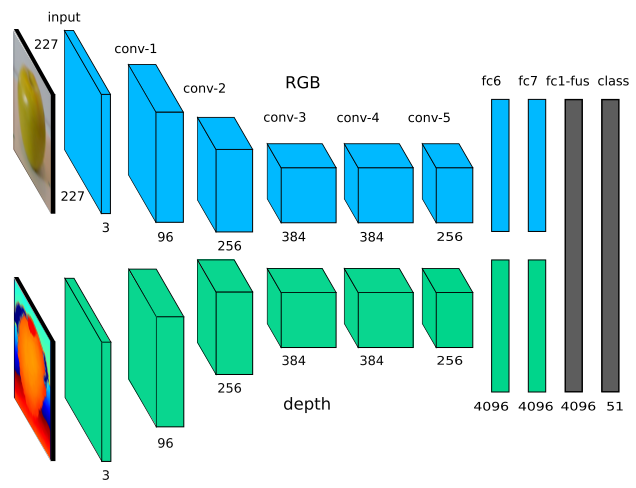
\includegraphics[width=\linewidth]{img/architecture.png} 
\caption{Network architecture using separate color and depth inputs. Inputs for color and depth are $227 \times 227 \times 3$, assuming depth colorization during preprocessing stage. Each modality has its own individual network, with the two resultant fusion layers providing final classification.}
\label{fig:network}
\end{figure}

\begin{figure}
    \centering
    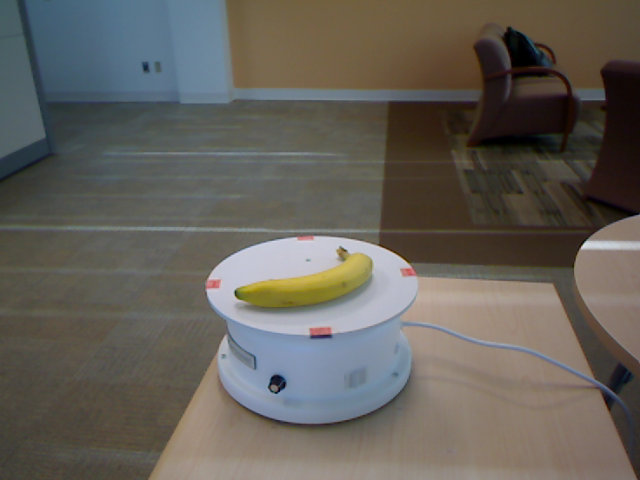
\includegraphics[width=0.7\linewidth]{img/banana_1_1_1.png}

    \vspace{0.4cm}
    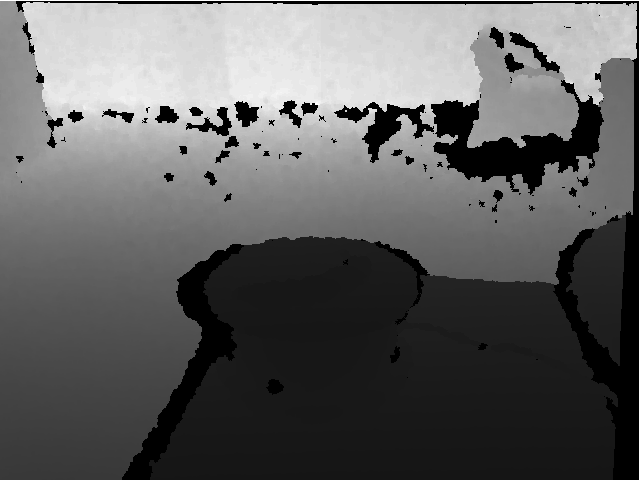
\includegraphics[width=0.7\linewidth]{img/banana_1_1_1_depth.png}
    \caption{Original color and depth photos of object captured on a turntable.}
    \label{fig:orig_img}
\end{figure}

\begin{figure}
    \centering
    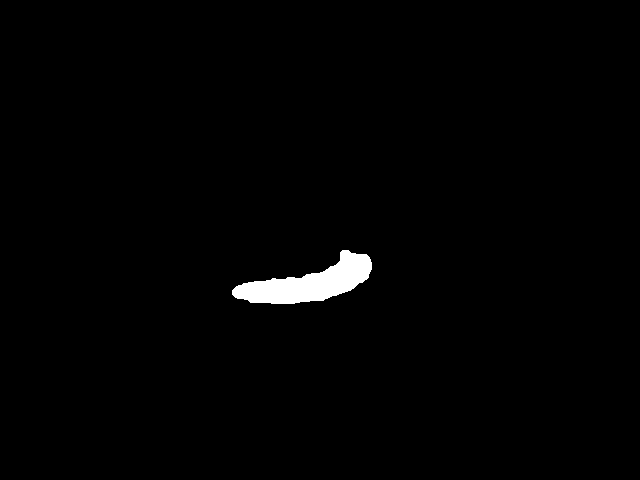
\includegraphics[width=0.7\linewidth]{img/banana_1_1_1_mask.png}
    \caption{Ground-truth segmentation mask for banana object.}
    \label{fig:img_mask}
\end{figure}

\begin{figure}
    \centering
    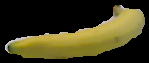
\includegraphics[width=0.7\linewidth]{img/banana_1_1_1_crop.png}

    \vspace{0.4cm}
    
\includegraphics[width=0.7\linewidth]{img/banana_1_1_1_depth_crop.png}
    \caption{Cropped banana photo using given segmentation mask.}
    \label{fig:img_cropped}
\end{figure}

\begin{figure}
    \centering
    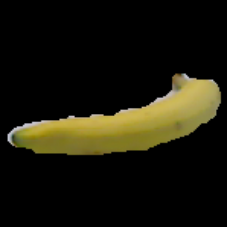
\includegraphics[width=0.7\linewidth]{img/banana_1_1_1_resize.png}

    \vspace{0.4cm}
    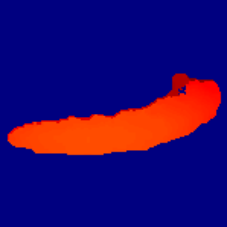
\includegraphics[width=0.7\linewidth]{img/banana_1_1_1_depth_resize.png} 
    \caption{Rescaled cropped color photo (top) and rescaled cropped depth photo (bottom) colorized using \textit{Jet} heatmap.}
    \label{fig:depth_colorized}
\end{figure}